\chapter{Generando UFO files con \textsc{FeynRules}}\label{GenUFO}

Para cargar un modelo en \textsc{FeynRules} se debe cargar el paquete en una sesión de \textsc{Mathematica}. Esto debe hacerse antes de que la descripción del modelo se cargue en el kernel, por lo que debe ser la primera línea del notebook de \textsc{Mathematica}. Para cargar \textsc{FeynRules}, el usuario primero debe especificar el directorio donde está almacenado y luego cargarlo usando 
%
\begin{verbatim}
$$ FeynRulesPath = SetDirectory[<La direccion del paquete>];
<< FeynRules'
\end{verbatim}
%
Por ejemplo, si el paquete se encuentra en el \verb|/home| se usa:
%
\begin{verbatim}
$$ FeynRulesPath = SetDirectory["~/feynrules-directorio"];
<< FeynRules'
SetDirectory["~/feynrules-directorio/Models/"];
\end{verbatim}
%
El \verb|SetDirectory| hace referencia a la ubicación donde buscará el modelo en el momento de cargarlo. Después de cargar el paquete de \textsc{FeynRules}, se puede cargar el modelo usando el comando 
%
\begin{verbatim}
LoadModel[<archivo.fr>, <archivo2.fr>, ...];
\end{verbatim}
%
Para que \textsc{FeynRules} corra adecuadamente, la extensión de los archivos debe ser \textbf{.fr}. \textsc{FeynRules} tiene la ventaja de poder almacenar el modelo en un solo archivo o en varios. Por ejemplo, si se quiere hacer una extensión al Modelo Estándar solo es necesario agregar el archivo adicional que genere la extensión. De esta forma el modelo se carga así:
%
\begin{verbatim}
LoadModel["sm.fr", "WZPrime.fr"];
\end{verbatim}
%
Cada vez que el modelo cambie, se debe volver a cargar.
Ahora, ya que se tiene cargado el modelo, \textsc{FeynRules} posee una variedad de comandos que permiten obtener los vértices, las reglas de Feynman asociados al lagrangiano, los parámetros del modelo, etc.  Dichos comandos y una descripción más detalladas se pueden encontrar en~\cite{Alloul:2013bka}. 

Una vez se han obtenido las reglas de Feynman, el usuario generalmente está interesado en la fenomenología del modelo, que requiere la evaluación de los diagramas de Feynman. Hay muchas herramientas que permiten evaluar diagramas de Feynman automáticamente. Si bien estas herramientas son en general muy flexibles y permiten al usuario generar, al menos en principio, diagramas de Feynman para cualquier proceso que satisfaga los requisitos básicos de la teoría cuántica de campos, la mayoría de las herramientas requieren una trabajo tedioso y propenso a errores para la implementación de estos.

\textsc{FeynRules} da la posibilidad de obtener salidas para varias interfaces. Actualmente \textsc{FeynRules} genera salidas para las siguientes interfaces,
\begin{itemize}
\item CalcHep/CompHep
\item FeynArts/FormCalc
\item Sherpa
\item UFO (Universal FeynRules output)
\item Whizard/Omega
\end{itemize}

El formato UFO es un formato de modelo genérico que almacena información del modelo de forma abstracta en forma de objetos Python para \textsc{MadGraph}. Todas las interfaces pueden ser invocadas con el comando 
%
\begin{verbatim}
WriteXOutput[L 1 ,L 2 ,. . . , options];
\end{verbatim}
%
donde $X$ es reemplazado con la etiqueta de referencia al nombre de cada interfaz. Las principales limitaciones de las interfaces se basan en el hecho de que solo se pueden usar para implementar partículas y vértices que son compatibles nativamente con el generador de diagramas de Feynman correspondiente. Ya que cada generador realiza suposiciones implícitas sobre las rotaciones o las representaciones de color de las partículas presentes en el modelo, y / o sobre la forma o la dimensión de los vértices de interacción. Como consecuencia, solo aquellos modelos que cumplen con todas esas restricciones son compatibles con una herramienta determinada. Las interfaces de \textsc{FeynRules} se adaptan a los diferentes generadores de diagramas de Feynman y, por lo tanto, permiten verificar caso por caso si un modelo dado cumple o no con una herramienta determinada. Por ejemplo, si una interfaz detecta que un vértice de interacción determinado no es compatible, el vértice se descarta y se imprime una advertencia en la pantalla. El usuario tiene la posibilidad de cambiar a un generador de diagramas Feynman diferente para el cual la restricción no está presente.

Si el interés es generar los UFO files necesarios para correr en \textsc{MadGraph} se debe ejecutar el siguiente comando
%
\begin{verbatim}
WriteUFO[<Lag1>, <Lag2>, …, Output -> "Carpeta", opciones];
\end{verbatim}
%
donde recibe como parámetros de entrada el lagrangiano de los diferentes archivos cargados en el notebook de \textsc{Mathematica}y la carpeta donde se quiere depositar los UFO files. En general se ejecuta  
%
\begin{verbatim}
WriteUFO[LFull, Output -> "UFO_files_output"];
\end{verbatim}
%
Tenga en cuenta que para que los archivos UFO funcionen correctamente, se debe asignar a todas las constantes de acoplamiento una orden de interacción.. En general se ejecuta
\newpage
\chapter{Modelo en \textsc{FeynRules}}\label{FeynRModel}
La implementación del modelo en \textsc{FeynRules} es:
\begin{verbatim}
(* ********************************************************* *)
(* *****                                               ***** *)
(* *****  FeynRules model file: SM + W&Z prime	       ***** *)
(* *****  Original Author:  M. Abdullah                ***** *)
(* *****                                               ***** *)
(* ********************************************************* *)

(* ************************** *)
(* *****  Information   ***** *)
(* ************************** *)
M$ModelName = "WZPrime";
M$Information = { Authors->{"M. Abdullah"}, 
		  Emails->{"mabdullah@tamu.edu"}, 
		  Institutions->{"Texas A&M University"},
          Date->"2017 Jan 11", 
		  Version->"1.0"};
FeynmanGauge = True;

(* ************************** *)
(* *****     Fields     ***** *)
(* ************************** *)
M$ClassesDescription = {
(* W prime boson *)
  V[34] == {
	ClassName        -> Wp,
	SelfConjugate    -> False,
	Mass             -> {MWp,  500.00},
	Width            -> {WWp,    50},
	ParticleName     -> "Wp+",
	AntiParticleName -> "Wp-",
    QuantumNumbers   -> {Q -> 1},
	PDG              -> 34, 
	PropagatorLabel  -> "Wp",
	PropagatorType   -> Sine,
	PropagatorArrow  -> None,
	FullName         -> "Wp"
  },

(* Z prime boson *)
  V[32] == {
	ClassName        -> Zp,
	SelfConjugate    -> True,
	Mass             -> {MZp,  500.00},
	Width            -> {WZp,    50},
	ParticleName     -> "Zp",
	PDG              -> 32, 
	PropagatorLabel  -> "Zp",
	PropagatorType   -> Sine,
	PropagatorArrow  -> None,
	FullName         -> "Zp"
  }
};

(* ************************** *)
(* *****   Parameters   ***** *)
(* ************************** *)
M$Parameters = {
  gb == { ParameterType -> External, 
	  Value -> 0.1,
	  InteractionOrder -> {BSM, 1},
	  BlockName->ZprimeCouplings,
	  TeX -> Subscript[g,b], 
          Description -> "Z' coupling to 3rd gen quarks"
	},

  gmu == { ParameterType -> External, 
	  Value -> 0.1,
	  InteractionOrder -> {BSM, 1}, 
	  TeX -> Subscript[g,mu], 
	  BlockName->ZprimeCouplings,
          Description -> "Z' coupling to 2nd gen leptons"
	},
	
	gtau == { ParameterType -> External, 
	  Value -> 0.1,
	  InteractionOrder -> {BSM, 1}, 
	  TeX -> Subscript[g,tau], 
	  BlockName->ZprimeCouplings,
          Description -> "Z' coupling to 3rd gen leptons"
	},
	
	delbs == { ParameterType -> External, 
	  Value -> 1.0,
	  InteractionOrder -> {BSM, 0}, 
	  TeX -> Subscript[delta,bs], 
	  BlockName->ZprimeCouplings,
          Description -> "Z' coupling scale factor to b and s quarks"
	},
	
	gwp == {ParameterType -> External,
	Value -> 0.1,
	InteractionOrder -> {BSM,1},
	TeX -> Subscript[g,wp],
	Description -> "W' coupling",
	BlockName->WprimeCoupling,
	Description-> "W' coupling"
	},
	
	Vcb == { ParameterType -> Internal,
	Value -> 0.0412,
	InteractionOrder -> {BSM,0},
	TeX -> Subscript[V,cb],
	Description -> "c-b CKM mixing"
	}

};

(* ******************************* *)
(* *****   BSM Lagrangians   ***** *)
(* ******************************* *)

LZQ := gb*Zp[mu]*( tbar.Ga[mu].ProjM.t \
			   +  bbar.Ga[mu].ProjM.b \
			   + delbs*sbar.Ga[mu].ProjM.b \
			   +HC[delbs*sbar.Ga[mu].ProjM.b]);
			   
LZL := 			gmu*Zp[mu]*(mubar.Ga[mu].mu \
				+vmbar.Ga[mu].ProjM.vm)\
				+gtau*Zp[mu]*(tabar.Ga[mu].ta \
				+vtbar.Ga[mu].ProjM.vt);
				
LW  := gwp*(Wp[mu]*cbar.Ga[mu].ProjM.b \
		+HC[Wp[mu]*cbar.Ga[mu].ProjM.b] \
		+Wp[mu]*vtbar.Ga[mu].ProjM.ta \
		+HC[Wp[mu]*vtbar.Ga[mu].ProjM.ta]);

(* Combine Everything *)

LFull := LSM + LZQ + LZL + LW;
\end{verbatim}
\newpage
\chapter{Generación de eventos en \textsc{MadGraph}}\label{GenMG}
Para cargar un modelo en \textsc{MadGraph}, primero se debe certificar que la carpeta con los archivos UFO se encuentre en la carpeta \textsc{models}. Luego se debe ejecutar el comando 
%
\begin{verbatim}
MG5_aMC> import model [directorio_del_modelo]
\end{verbatim}
%
Después de esto se deben de definir los eventos a generar. Se comienza definiendo los estados iniciales en el evento, separados de los estados finales por “\textgreater”. Para generación de procesos partónicos se utiliza el comando 
%
\begin{verbatim}
MG5_aMC> generate p p > S
\end{verbatim}
%
donde $S$ hace referencia a todas las partículas en el estado final, sin incluir partones ligeros de QCD, ni quarks b (y que no incluye partículas BSM cargadas bajo QCD). Si se desea adicionar procesos a la generación de eventos se ejecuta el siguiente comando
%
\begin{verbatim}
MG5_aMC> add process p p > S1
\end{verbatim}
%
donde $S1$ hace referencia a un conjunto diferentes de partículas en el estado final anterior.
Además, si se quiere adicionar jets ($j$), sólo se necesita adicionar $j$ a los estados finales. Por ejemplo, para adicionar eventos con dos jets se ejecuta el siguiente comando
%
\begin{verbatim}
MG5_aMC> add process p p > S j j
\end{verbatim}
%
Luego de tener los procesos para generar los eventos, se debe almacenar la salida de dichos eventos para la ejecución. Para esto se ejecuta el comando
%
\begin{verbatim}
MG5_aMC> output [directo_de_salida] -f
\end{verbatim}
%
Si el directorio no existe lo crea, de lo contrario, si el directorio existe la bandera \verb|-f| se utiliza para borrar todos los archivos en estos. 

Antes de realizar la ejecución se deben definir los diferentes parámetros de la generación de eventos. En \textsc{MadGraph} los parámetros se configuran de las tarjetas de configuración. Todas éstas tarjetas de configuración se pueden encontrar en el directorio \verb|Cards| en el directorio de salida generado por \textsc{MadGraph}. La \verb|proc_card|, es dónde se declaran los procesos a generar. Esta tarjeta se genera automáticamente y su modificación no tiene efecto alguno. La \verb|param_card|, es la tarjeta donde se controla el valor de los parámetros del modelo. La \verb|run_card|, permite controlar los parámetros de la simulación, por ejemplo, el número de eventos a generar.

Luego de tener la configuración que se desea, se deben ejecutar los procesos anteriormente generados. Para esto se utiliza el comando
%
\begin{verbatim}
MG5_aMC> launch [directo_de_salida]
\end{verbatim}
%
Después de esto vemos la interfaz de MadGraph~\ref{Fig:IMG}, donde preguntan por los programas para las diferentes simulaciones de los procesos. 
%
\begin{figure}
\begin{center}
\begin{verbatim}
The following switches determine which programs are run:
/--------------------------------------------------------------------------------\
|  1. Choose the shower/hadronization program:           shower = PYTHIA8      |
|  2. Choose the detector simulation program:            detector = OFF        |
|  3. Run an analysis package on the events generated:   analysis = No analysis 
tool interfaced to MG5aMC.|
|  4. Decay particles with the MadSpin module:		      	   madspin = OFF         |
|  5. Add weights to events for different model hypothesis:		   reweight = OFF              |
/--------------------------------------------------------------------------------\
\end{verbatim}
\caption{Interfaz de MadGraph. Se preguntan por los programas requeridos para simulaciones requeridas en los procesos.}
\label{Fig:IMG}
\end{center}
\end{figure}
%
Para realizar la simulación del proceso de hadronización sobre el proceso partónico se utiliza Pythia 8. 

Para realizar simulaciones con jets adicionales se debe de realizar el proceso de \textbf{merging}. Este proceso consiste de la separación del espacio de parámetros que es simulado por \textsc{MadGraph} y por Pythia. \textsc{MadGraph} debe encargarse solo de los jets “duros” (con gran cantidad de momento) y Pythia se debe encargar de los jets “suaves” (con baja cantidad de momento). Para garantizar el \textbf{merging} se deben definir los valores de \textbf{xqcut} para MadGraph y \textbf{qcut} Pythia. 

Para encontrar los valores óptimos de las variables de \textbf{merging}, para cada valor de \textbf{xqcut} se debe realizar un escaneo sobre \textbf{qcut} (teniendo en cuenta que \textbf{xqcut} \textless \textbf{qcut}) hasta encontrar el valor que estabilice la sección eficaz. La optimización cambia de acuerdo a los procesos, el número de jets adicionales incluidos y/o los cortes cinemáticos.

\chapter{Comparación LO vs NLO}\label{LOvsNLO}

\begin{table}[htbp]
\begin{center}
\begin{tabular}{clll}\hline
$M_{W^{\prime}}$ [GeV] &               $\sigma_{LO}$ [Pb] &             $\sigma_{NLO}$ [Pb] & Cambio relativo \\\hline
200  &   $30.38$ &    $35.07 $ &    $15.43\%$ \\
700 &    $0.1654$ &   $0.1796 $ &   $8.58\%$ \\
1000 &   $0.02603$ &  $0.02778 $ &  $6.7\%$ \\\hline
\end{tabular}
\caption {Comparación de sección eficaz para procesos generados a orden principal (LO) y a segundo orden (NLO).}
\label{tab:cutefficiencynw}
\end{center}
\end{table}
%


%
\begin{figure}
\begin{center}
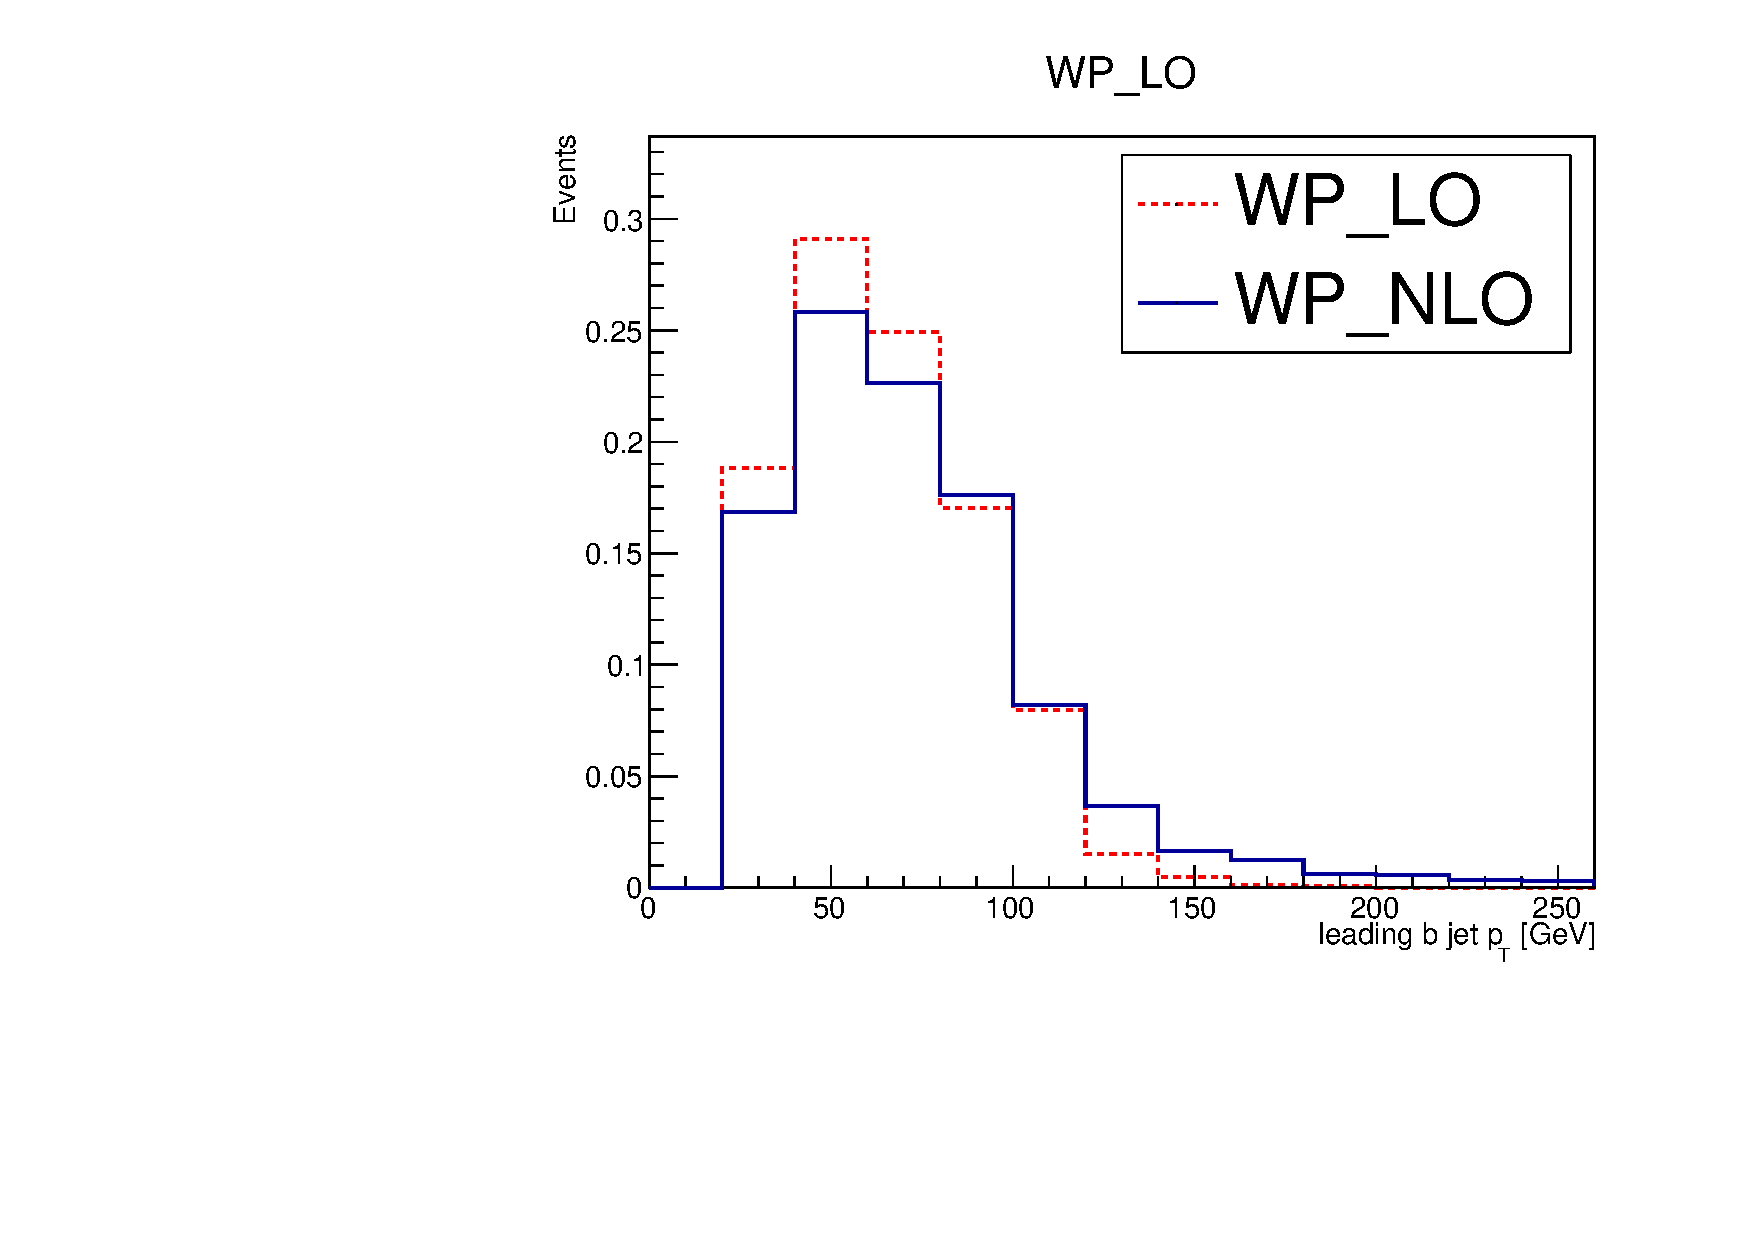
\includegraphics[width = 0.45 \textwidth]{figures/leading_jet_p_T_200_Norm.pdf}
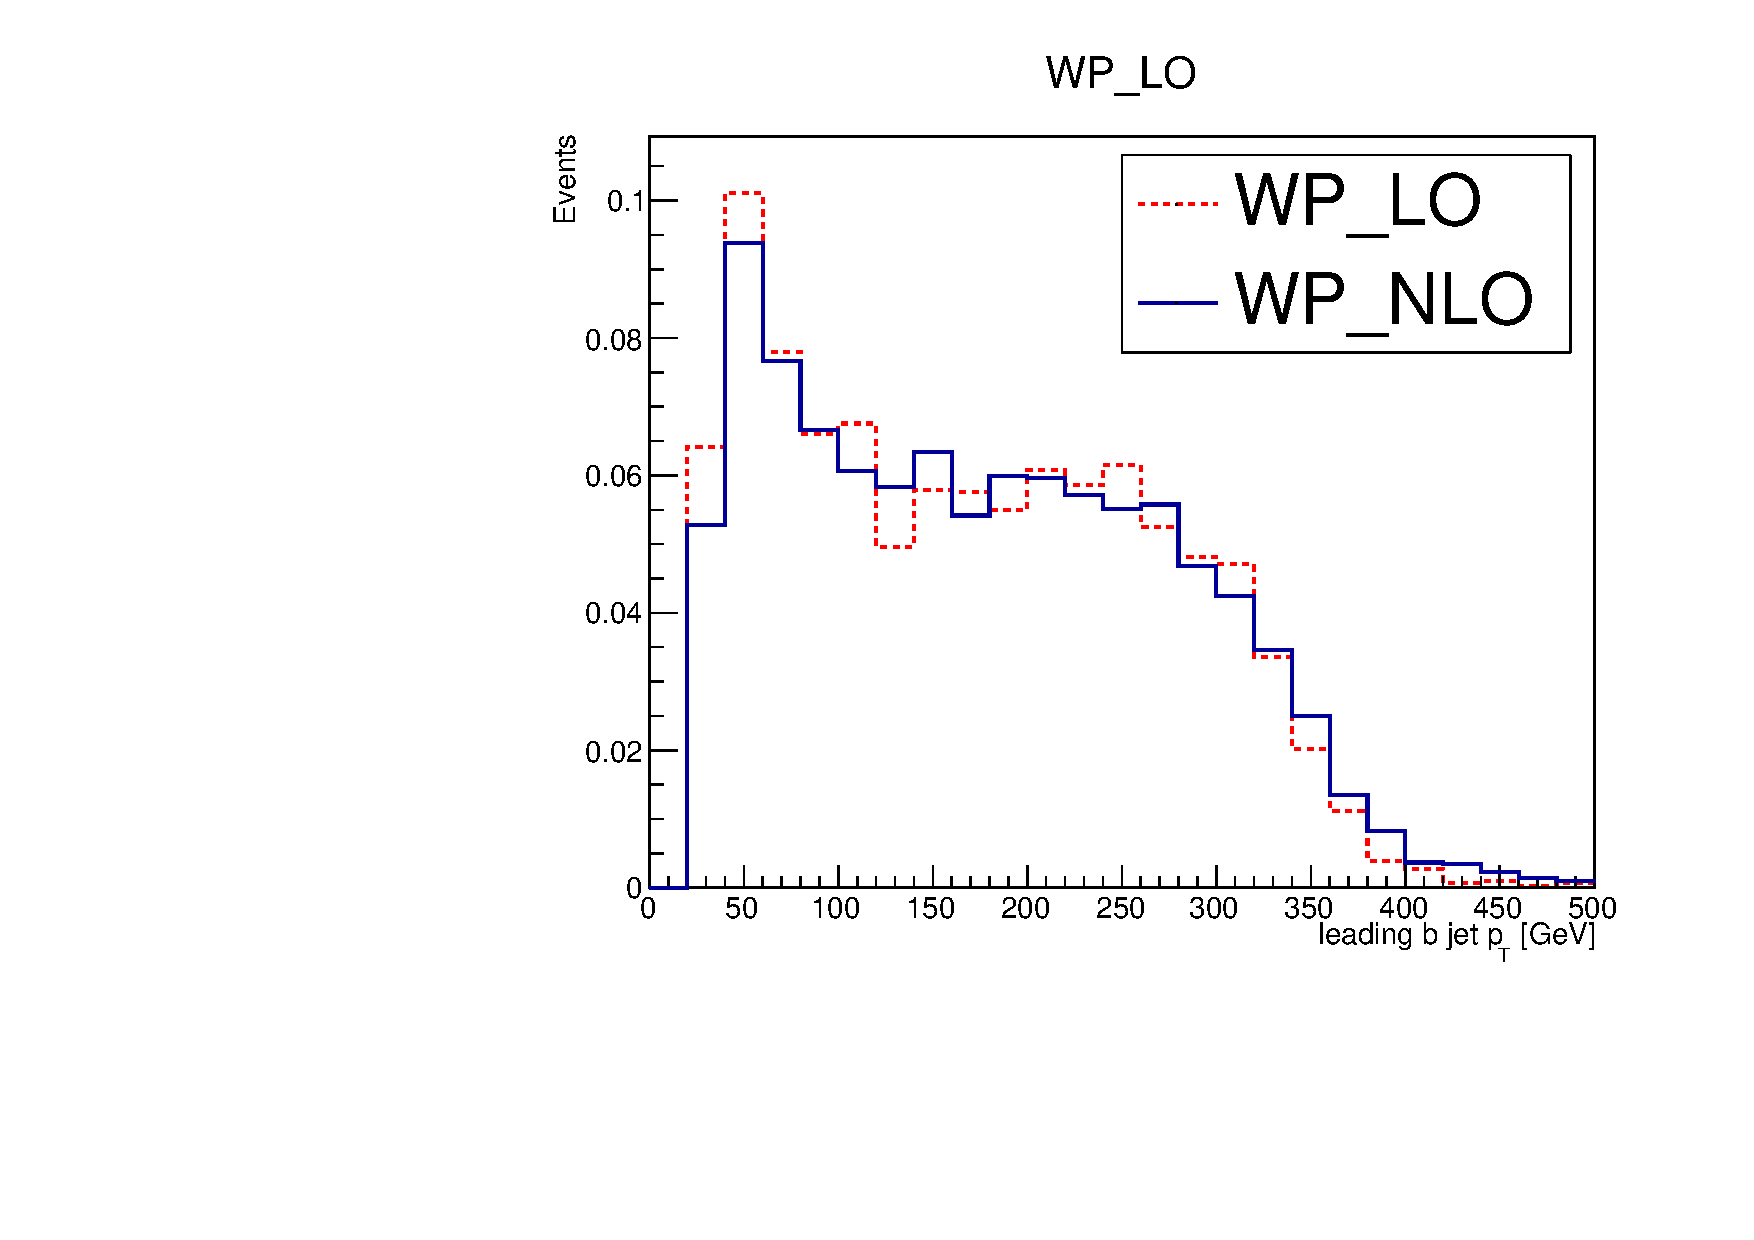
\includegraphics[width = 0.45 \textwidth]{figures/leading_jet_p_T_700_Norm.pdf}
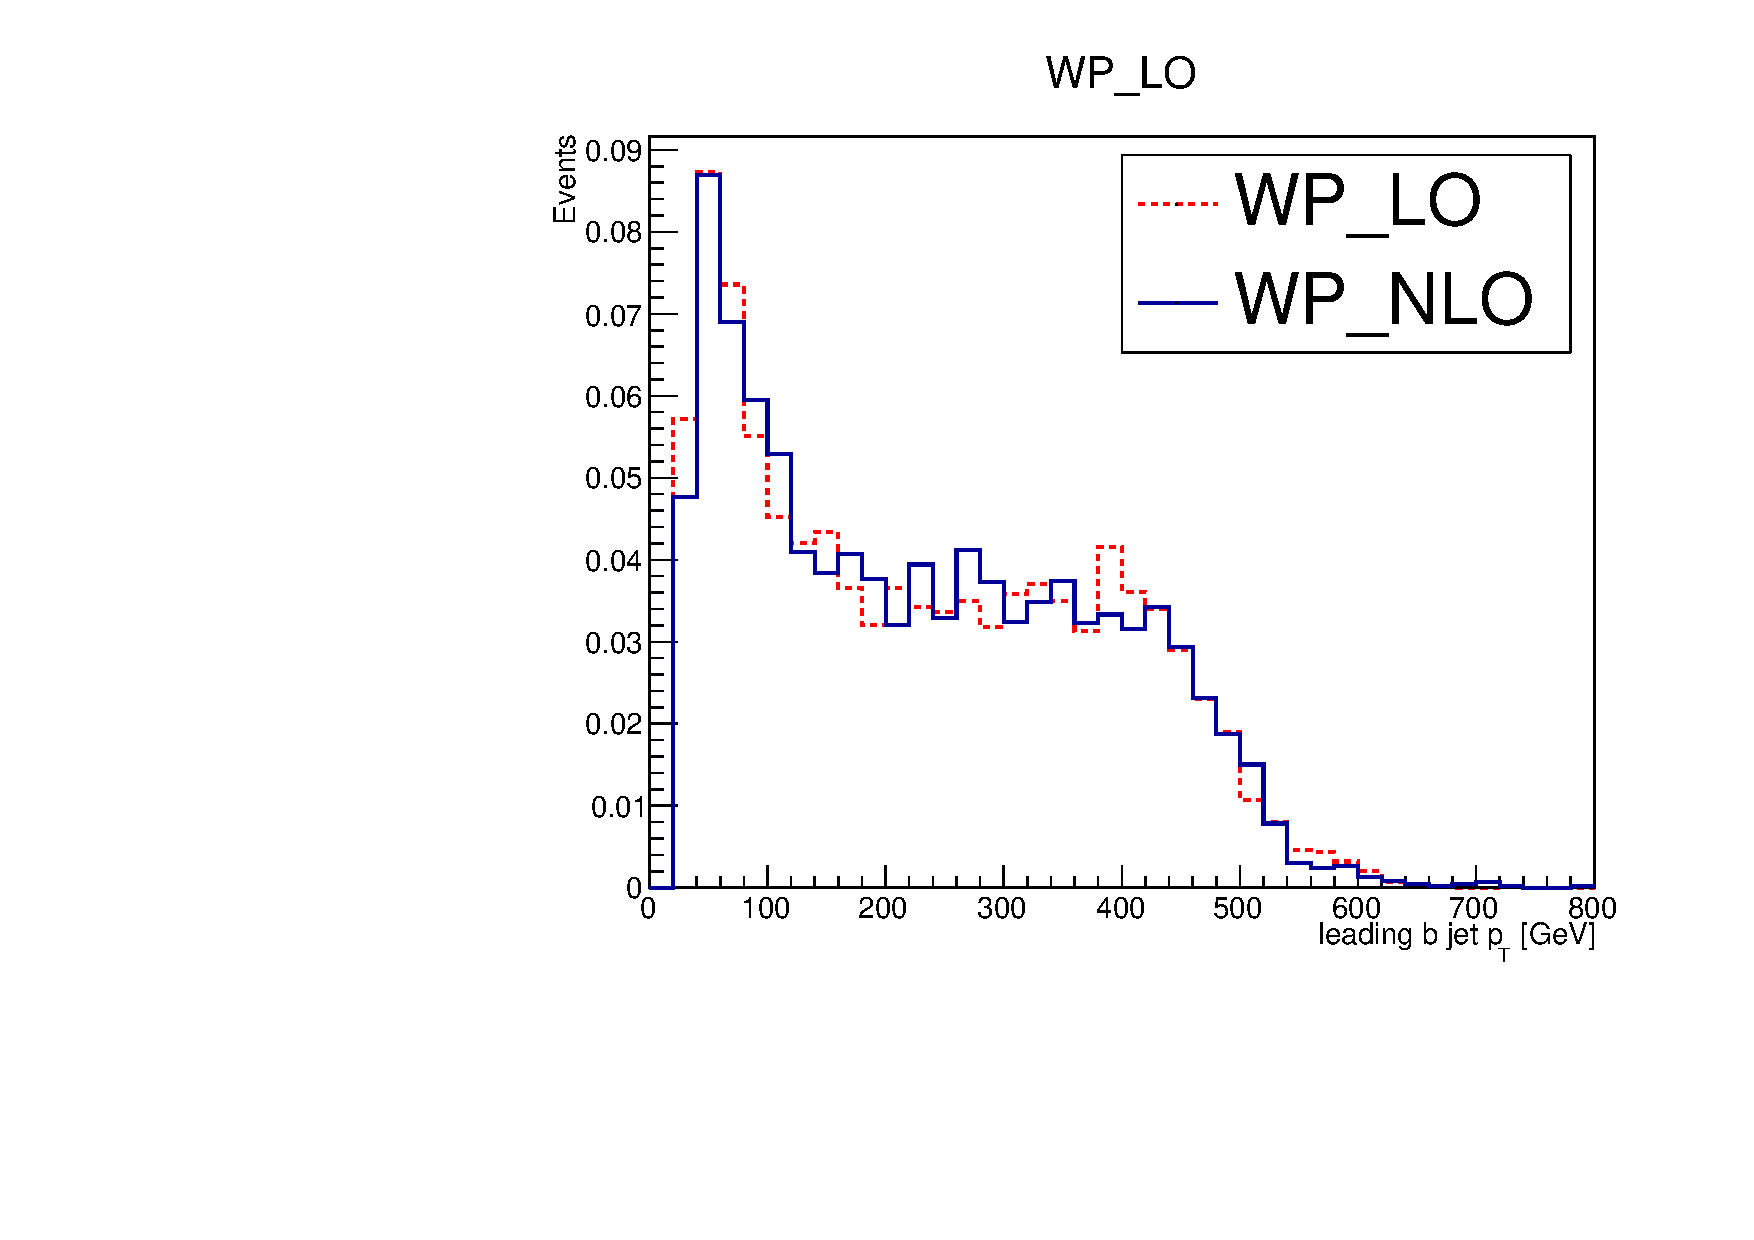
\includegraphics[width = 0.45 \textwidth]{figures/leading_jet_p_T_1000_Norm.pdf}
\caption{Distribución de $p_{T}$ para el jet $b$ principal para $M_{W^{\prime}} = 200$ GeV (superios izquierda), $M_{W^{\prime}} = 700$ GeV (superior derecha) y $M_{W^{\prime}} = 1000$ GeV (inferior). Aquí no se ve un cambio significativo en la distribución de $p_{T}$ para los eventos simulados a orden principal (LO) y a segundo orden (NLO).  }
\label{Fig:DisCine}
\end{center}
\end{figure}
%